\chapter{Grundlagen} % (fold)
\label{sec:grundlagen}
Das vorliegende Kapitel vermittelt die theoretischen Grundlagen für das Verständnis dieser Arbeit. Dabei umfassen die hier beschriebenen Konzepte relationale Algebra, Graphentheorie, APIs sowie relationale und Graphdatenbanken.
\section{Relationale Algebra} % (fold)
\label{sec:relationaleAlgebra}
Die relationale Algebra beschreibt ein mathematisches System, das 1970 von E. F. Codd entwickelt wurde und unter anderem zur Abfrage sowie Mutation von Daten in relationalen Datenbanken verwendet wird. Durch die relationale Algebra wird eine Menge an Operationen beschrieben, die auf Relationen angewendet werden können, um neue Relationen zu bilden.  \citep{relationalModel}

\subsection{Basisrelation} % fold
\label{sec:basisrelation}
Die Anwendung relationaler Algebra erfordert die Verwendung von Basisrelationen als fundamentale Bausteine, um mittels Grundoperationen komplexe Ausdrücke zu konstruieren, die neue Relationen definieren. Eine Basisrelation setzt sich aus drei Komponenten zusammen: Tupel, Attributen und Domänen. Tupel reflektieren die Zeilen einer Tabelle, die die einzelnen Datensätze repräsentieren. Diese werden durch Attribute in spezifische Spalten eingeteilt, worin die Eigenschaften der Tupel beschrieben sind. Die für die einzelnen Attribute zulässigen Wertebereiche werden als Domänen bezeichnet. Demnach entspricht jede Relation einer Menge von Tupeln mit spezifischen Attributen sowie deren Domänen. \citep{rdb}
%subsection basisrelation (end)

\subsection{Grundoperationen} % fold
\label{sec:grundoperationen}
Grundoperationen in der relationalen Algebra beschreiben einfache mengentheoretische Operationen, die auf die Basisrelationen angewandt werden. Insgesamt existieren sechs Grundoperationen, die nachfolgend erläutert werden.
\begin{itemize}
\item Bei der \textbf{Selektion $\sigma$}werden die einzelnen Tupel basierend auf einer Bedingung gefiltert, beispielsweise \colorbox{gray!20}{$\sigma$ Alter > 30 (Person)}. Hierdurch werden nur Personen mit einem Alter von über 30 Jahren zurückgeliefert.
\item Die \textbf{Projektion $\pi$} ermöglicht die Auswahl oder Entfernung bestimmter Attribute einer Relation. Beispielsweise werden durch \colorbox{gray!20}{$\pi$ Name, Alter (Person)} nur der Name und das Alter einer Person zurückgegeben. 
\item Das \textbf{Kartesische Produkt $\times$} kombiniert jede Zeile der ersten mit jeder Zeile der zweiten Relation, womit  \colorbox{gray!20}{$R \times S$} alle möglichen Kombinationen aus \colorbox{gray!20}{R} und \colorbox{gray!20}{S} erzeugt.
\item Eine \textbf{Vereinigung $\cup$}verknüpft die Tupel zweier Relationen, die dieselbe Struktur aufweisen. \colorbox{gray!20}{$R \cup S$}kombiniert somit alle Tupel aus beiden Relationen mit identischer Struktur, ohne Duplikate zu erzeugen.
\item Weiter liefert die  \textbf{Differenz  $\setminus$} zweier Relationen alle Tupel, die in der ersten Relation vorkommen, aber nicht in der zweiten. Somit gibt 
 \colorbox{gray!20}{$R \setminus S$} alle Tupel \colorbox{gray!20}{R} aus, die nicht in \colorbox{gray!20}{S} enthalten sind.
\item Der \textbf{Schnitt $\cap$}nennt die Tupel, die in beiden Relationen vorhanden sind. Somit gibt \colorbox{gray!20}{$R \cap S$} die Tupel zurück, die sowohl in \colorbox{gray!20}{R} als auch in \colorbox{gray!20}{S} enthalten sind.
\end{itemize}
\noindent Durch die Verbindung dieser Grundoperationen können andere Operationen erstellt werden, beispielsweise ein Theta-Join $\bowtie$, der durch eine Kombination aus kartesischem Produkt und Selektion alle Tupel zweier Relationen aufgrund einer Bedingung zusammenlegt. \citep{rdb}
%subsection grundoperationen (end)
% section relationaleAlgebra (end)

\section{Graphentheorie} % (fold)
\label{sec:graphentheorie}
Ein Graph besteht im Allgemeinen aus Knoten und verbindenden Kanten (vgl. Abb 2.1). In der Informatik bietet diese Datenstruktur einen deutlichen Vorteil gegenüber der relationalen Algebra, wenn stark verzweigte Daten vorliegen.  \citep{graphTheory}

\begin{figure}[h!]
	\centering
	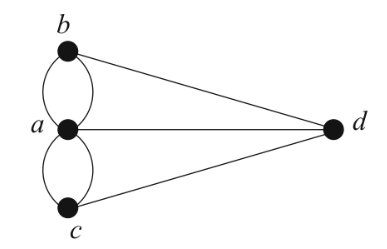
\includegraphics[scale=1]{Illustrations/graph.png}
	\caption{Modell eines ungerichteten Graphen. \citep{graphTheory}}
\end{figure}
\newpage
\subsection{Knoten} % fold
\label{sec:knoten}
Knoten beschreiben Punkte innerhalb eines Graphen, die beispielsweise als Objekte der realen Welt verstanden werden können. Sie können zum Beispiel als geografische Koordinaten dienen, um einen Distanzgraphen zu erstellen, oder als Webseiten, um einen Webgraphen zu erhalten, der die Verbindung verschiedener Webseiten aufzeigt. Innerhalb der Knoten werden verschiedene Typen unterschieden: Zum einen existieren isolierte Knoten ohne Verbindung zu anderen Knoten des Graphen, die zur Identifizierung nicht verbundener Teile eines Netzwerks verwendet werden können. Zum anderen bestehen verbundene Knoten, die mindestens eine Verbindung zu einem anderen benachbarten Knoten aufweisen. Außerdem kann eine indirekte Verbindung entstehen, indem ein Pfad zwischen Ausgangs- und Endknoten existiert, der über mehrere Verbindungen führt.  \citep{graphTheory} \citep{graphapplication}
%subsection knoten (end)

\subsection{Kanten} % fold
\label{sec:kanten}
Kanten dienen in einem Graphen dazu, Knoten miteinander zu verbinden, um eine Relation zwischen ihnen zu visualisieren. Jede Kante besitzt einen Start- und Endknoten, wobei es sich um denselben Knoten handelt kann; in diesem Fall liegt eine Schleife vor. Ebenso wie es verschiedene Arten von Knoten gibt, existieren auch verschiedene Kanten. 
In Abb. 2.1 sind \textit{ungerichtete Kanten}im Graphen zu sehen, Sie die die Knoten auf die trivialste Art verbinden, indem sie ohne Richtung, Gewicht oder andere Beschränkung eine Verbindung herstellen. Durch ungerichtete Kanten entsteht ein ungerichteter Graph. 
\textit{Gerichtete Kanten} werden in Abb. 2.2 (a) durch einen Pfeil visualisiert, der angibt, in welche Richtung der Graph eine Beziehung zwischen den Knoten herstellt. Es ist ebenfalls möglich, dass zwei Knoten eine beidseitige Beziehung durch zwei gerichtete Kanten eingehen, also eine Kante pro Richtung. Ein Graph, der durch gerichtete Kanten verbunden ist, wird ‚gerichteter Graph‘ genannt. Werden Zahlenwerte zu einer Kante hinzugefügt (vgl. Abb 2 (b)), so handelt es sich um eine \textit{gewichteten Kante}. Sie können verwendet werden, um die Strecke zwischen zwei Kanten darzustellen oder die Kosten für die Nutzung der Kante anzugeben. Wird ein Graph mit gewichteten Kanten verbunden, liegt ein gewichteter Graph vor. \citep{graphTheory} \citep{graphapplication}
\begin{figure}[H]
	\centering
	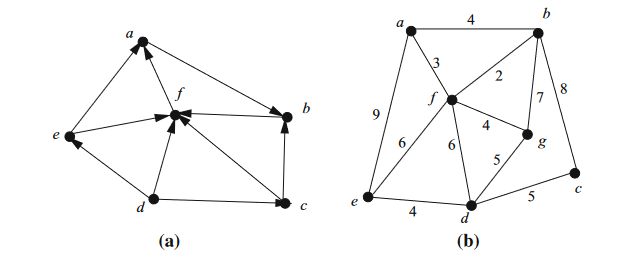
\includegraphics[scale=1]{Illustrations/graph_01.png}
	\caption{Modell eines gerichteten (a) und eines gewichteten Graphen (b). \citep{graphTheory}}
\end{figure}
%subsection kanten (end)

\subsection{Traversierung} % fold
\label{sec:traversierung}
Die Bewegung eines Knoten oder einer Kante zu einem anderen Knoten innerhalb eines Graphen nach vorgegebenen Kriterien wird als Traversierung bezeichnet. Graphdatenbanken bieten in der Regel Traversierungsmechanismen, um Daten miteinander verbundener Knoten effizient abzufragen sowie abzurufen. \cite{graph}
%subsection traversierung (end)


% section graphentheorie (end)

\section{APIs} % (fold)
\label{sec:apigrundlagen}
Nachfolgend werden die Grundlagen von APIs erläutert, wobei die grundlegenden Definitionen sowie die für diese Arbeit relevanten Typen behandelt werden.
\subsection{Definition} % (fold)
\label{sec:grundlegendedefinitionvonapi}
Eine API bezeichnet eine Schnittstelle, die Entwicklern den Zugriff auf Daten und Informationen ermöglicht. Beispiele für häufig genutzte APIs bieten die Twitter- und Facebook-APIs, die für Entwickler zugänglich sind und die Interaktion mit der Software von Twitter sowie Facebook ermöglichen. Zudem erlauben APIs die Kommunikation zwischen Anwendungen und bieten diesen einen Weg, miteinander über ein Netzwerk, überwiegend das Internet, in einer gemeinsamen Sprache zu kommunizieren.  \citep{apistrategyguide}
%subsection grundlegendedefinitionvonapi (end)
\newpage
\subsection{REST API} % (fold)
\label{sec:restapi}
 \textbf{REST} wurde erstmals im Jahr 2000 in einer Dissertation von Roy Fielding beschrieben, wobei es sich um einen Software-Architekturstil für APIs handelt. Dabei basiert REST auf dem ressourcenorientierten Designprinzip, wonach jede Entität als Ressource betrachtet und durch einen eindeutigen Uniform Resource Locator identifiziert wird. Die Architektur fundiert auf sechs grundlegenden Beschränkungen, der Client-Server-Architektur, der Zustandslosigkeit, dem Caching, der einheitlichen Schnittstelle, dem Mehrschichtigen Systemmodell sowie dem Code on Demand. Die Client-Server-Architektur beschreibt, dass der Client und Server unabhängig voneinander agieren. Einen wesentlichen Bestandteil von REST bildet die Zustandslosigkeit, d. h., jede Anfrage beinhaltet sämtliche für die Verarbeitung erforderlichen Informationen, was die Interaktion zwischen Client und Server vereinfacht. Die Umsetzung der Operationen Create, Read, Update und Delete (CRUD) erfolgt durch die HTTP-Methoden (POST, GET, PUT, DELETE). Das in HTTP integrierte Caching nutzt REST, um die Antwortzeiten und die Leistung zu optimieren, wobei die Möglichkeit besteht, Serverantworten als cachefähig oder nicht cachefähig zu kennzeichnen. Des Weiteren ist eine einheitliche Schnittstelle zu nennen, die die Interaktionen zwischen unterschiedlichen Geräten und Anwendungen erleichtert, worüber hinaus REST ein mehrschichtiges System erfordert, bei dem jede Komponente lediglich mit der unmittelbar vorgelagerten Schicht interagiert. Code on Demand ist die letzte Einschränkung und besagt, dass Ressourcen bei der Antwort auf Anfragen darauf vorbereitet sind, Code bereitzustellen der auf dem Client und nicht auf dem Server ausgeführt wird. Diesen Prinzipien folgende RESTful-APIs, nutzen HTTP-Anfragen, um Ressourcen effizient zu bearbeiten.  \citep{Fielding2000}  \citep{graphqlreplacerest}

%subsection restapi (end) 
\subsection{GraphQL} % (fold)
\label{sec:graphql}
\textbf{GraphQL} wurde 2012 von Facebook für den internen Gebrauch entwickelt und 2015 als Open-Source-Projekt veröffentlicht. Das Kernkonzept von GraphQL basiert auf clientgetriebenen Abfragen, bei denen der Client die Struktur der Daten präzise definiert und nur die tatsächlich benötigten Daten anfordert. Diese clientseitige Steuerung reduziert die Menge der übertragenen Daten und führt zu effizienteren Netzwerkaufrufen, weil nur die relevanten Informationen übermittelt werden. Im Vergleich zu REST verursacht GraphQL signifikant weniger Overhead, was die Netzwerkperformance optimiert. Die hierarchische Struktur der Abfragen, die die Graphstruktur widerspiegelt, ermöglicht eine intuitive und flexible Datenmodellierung, wobei die starke Typisierung in GraphQL durch ein Schema definiert wird, das die Typen der Daten spezifiziert, was eine effizientere Validierung der Abfragen und eine klarere Dokumentation erlaubt. Im Gegensatz zu REST, der für verschiedene Operationen mehrere Endpunkte erfordert, nutzt GraphQL nur einen Endpunkt für alle API-Abfragen, was die Komplexität auf der Serverseite reduziert und eine vereinfachte API-Verwaltung ermöglicht. \citep{graphqlreplacerest}
%subsection graphql (end)
% section apigrundlagen (end)

\section{Datenbank} % (fold)
\label{sec:datenbankGrundlagen}
Im Folgenden werden die Grundlagen von Datenbanken behandelt, indem zentrale Definitionen im Zusammenhang mit Datenbanken und die verschiedenen Arten von Datenbanken vorgestellt werden.
\subsection{Definition von Datenbank und Datenbank-Management-System} % (fold)
\label{sec:definitiondatenbank}
Eine Datenbank stellt eine Sammlung von Daten und Informationen dar, die für den einfachen Zugriff gespeichert und organisiert werden, was sowohl die Verwaltung als auch die Aktualisierung der Daten umfasst. Die in der Datenbank gespeicherten Inhalte können nach Bedarf erweitert, gelöscht oder geändert werden. Dabei basiert die Funktionsweise von Datenbanksystemen auf der Abfrage von Informationen oder Daten, woraufhin entsprechende Anwendungen ausgeführt werden. Hier bezeichnet ‚Datenbank-Management-System‘ (DBMS) eine Systemsoftware, die für die Erstellung und Verwaltung von Datenbanken eingesetzt wird. Zu den Funktionalitäten zählen die Erstellung von Berichten, die Kontrolle von Lese- und Schreibvorgängen sowie die Durchführung einer Nutzungsanalyse. Das DBMS fungiert als Schnittstelle zwischen den Endnutzern und der Datenbank, um die Organisation und Manipulation von Daten zu erleichtern, wobei die Kernfunktionen des DBMS die Verwaltung von Daten, des Datenbankschemas, das die logische Struktur der Datenbank definiert, sowie der Datenbank-Engine umfassen, die das Abrufen, Aktualisieren und Sperren von Daten ermöglicht. Diese drei wesentlichen Elemente dienen der Bereitstellung standardisierter Verwaltungsverfahren, der Gleichzeitigkeit, der Wiederherstellung, der Sicherheit und der Datenintegrität.  \citep{9677042}

%subsubsection definitiondatenbank (end)

\subsection{Relationale Datenbank} % (fold)
\label{sec:relationaleDatenbanken}
Relationale Datenbanken basieren auf dem von E. F. Codd entwickelten relationalen Modell und fundieren auf relationaler Algebra sowie dem Tupel-Relational-Kalkül. Sie speichern Daten in einer hochstrukturierten Tabellenform, wobei jede Tabelle aus Zeilen, den sogenannten Tupeln, und Spalten, den sogenannten Attributen, besteht. Jede Zeile repräsentiert einen Datensatz, während jede Spalte durch einen spezifischen Datentyp definiert ist. Diese Struktur ermöglicht eine klare Organisation der Daten und erleichtert deren Verwaltung. Relationale Datenbanken verwenden Primär- und Fremdschlüssel, um Beziehungen zwischen Tabellen herzustellen sowie referenzielle Integrität zu gewährleisten, wodurch die Datenkonsistenz erhalten bleibt. Aufgrund dieser Eigenschaften werden die Tabellen auch als ‚Relationen‘ bezeichnet.

\newpage \noindent
Die bekanntesten relationalen Datenbank Management Systeme (RDBMS) sind Microsoft SQL Server, Oracle MySQL und IBM DB2. Ein RDBMS organisiert alle Daten in tabellarischer Form und bietet Funktionen wie Primärschlüssel zur eindeutigen Identifikation von Datensätzen sowie Indizes, die die Geschwindigkeit der Datenabfragen erhöhen. Darüber hinaus unterstützen RDBMS die Erstellung virtueller Tabellen, die komplexe Abfragen vereinfachen, sowie einen kontrollierten Mehrbenutzerzugriff mit individueller Rechtevergabe. Die Verwendung einer standardisierten SQL ermöglicht die Verwaltung, Abfrage und Manipulation von Daten, wobei die genannten Merkmale die Flexibilität und Benutzerfreundlichkeit relationaler Datenbanken stärken. Ein Vorteil relationaler Datenbanken liegt in ihrer Unterstützung der Prinzipien Atomicity, Consistency, Isolation und Durability (ACID), die Stabilität und Sicherheit bei Transaktionen gewährleisten, was sie für mehrere Anwendungsbereiche geeignet macht. Darüber hinaus bieten sie eine hohe Datenintegrität, reduzieren Redundanz und ermöglichen die einfache Implementierung von Sicherheitsmaßnahmen. Trotz dieser Vorteile stoßen relationale Datenbanken bei bestimmten Anforderungen an ihre Grenzen:. Sie sind selten für hohe Skalierbarkeit geeignet und können mit dem exponentiellen Wachstum von Daten schwer umgehen. Auch die Einrichtung und Wartung solcher Systeme erweist sich häufig als kostspielig und die Verwaltung unstrukturierter Daten wie Multimedia oder Social-Media-Inhalten stellt eine Herausforderung dar. Zudem erschwert die tabellarische Struktur komplexe Datenverknüpfungen und die Integration mehrerer Datenbanken. Aufgrund dieser Einschränkungen führten moderne Anwendungen und Big-Data-Anforderungen zur Entwicklung von NoSQL-Datenbanken, die effektiver auf die Verwaltung unstrukturierter und verteilter Daten ausgelegt sind. Dennoch bleiben relationale Datenbanken aufgrund ihrer Standardisierung, Benutzerfreundlichkeit und ihrer breiten Einsatzmöglichkeiten ein wesentlicher Bestandteil der Datenbanktechnologie.  \citep{relationalDatabase}  \citep{9677042}
%subsection relationaleDatenbanken (end)
\subsection{Graphdatenbanken} % (fold)
\label{sec:graphDatenbanken}
Graphdatenbanken beschreiben spezialisierte Datenbanksysteme, die dem User ein Datenmodell in Form eines Graphen präsentieren. Darüber hinaus enthalten die Graphen Informationen über die Eigenschaften der Knoten und Kanten, was eine flexible und schemafreie Speicherung semistrukturierter Daten ermöglicht. Abfragen in Graphdatenbanken wer- den häufig als Traversal formuliert, wodurch sie gegenüber relationalen Datenbanken erhebliche Geschwindigkeitsvorteile bieten, insbesondere bei komplexen Beziehungsabfragen. Es wird zwischen nativen und nicht nativen Graphdatenbanken unterschieden, wobei native Graphdatenbanken speziell für das Graphmodell entwickelt sind und die Daten intern in Graphenform speichern. Nicht native Graphdatenbanken hingegen verwenden andere Speichertechnologien, beispielsweise relationale Datenbanken, und präsentieren die Daten lediglich in Form von Graphen, um CRUD-Zugriffe zu ermöglichen. Beide Typen gehören zur Kategorie der NoSQL-Datenbanken, die durch den Verzicht auf das starre Tabellenschema relationaler Datenbanken deren Schwächen umgehen. Durch ihre besondere Architektur ermöglichen Graphdatenbanken nicht nur eine effiziente Verarbeitung von Beziehungsdaten, sondern erfüllen auch ACID-Bedingungen und unterstützen Rollbacks, was die Konsistenz der gespeicherten Informationen gewährleistet. Damit stellen sie eine leistungsstarke Alternative zu traditionellen relationalen Datenbanken dar, insbesondere in Anwendungsbereichen mit hochgradig verknüpften Daten. 
\citep{9677042} \citep{graphdb} 
%subsection graphDatenbanken (end)
% section datenbankGrundlagen (end)

% chapter grundlagen (end)